
\chapter{Methodology}
\section{ Project Management Model}

Our project began with a comprehensive requirements gathering phase where we collaborated closely with the client to define the project's scope. We established a set of core features for a \textbf{Minimum Viable Product (MVP)} \cite{atlassian_mvp}, which was formally documented and approved. This clear initial plan allowed us to structure the project efficiently while also outlining a roadmap for future enhancements. A key objective was to minimize dependencies among team members. To achieve this, we created a well-structured Product Requirements Document (PRD) \cite{atlassian_requirements} that enabled each team member to work on different components independently, fostering a parallel development process and ensuring a clear understanding of individual responsibilities.

\begin{figure}[h]
    \centering
    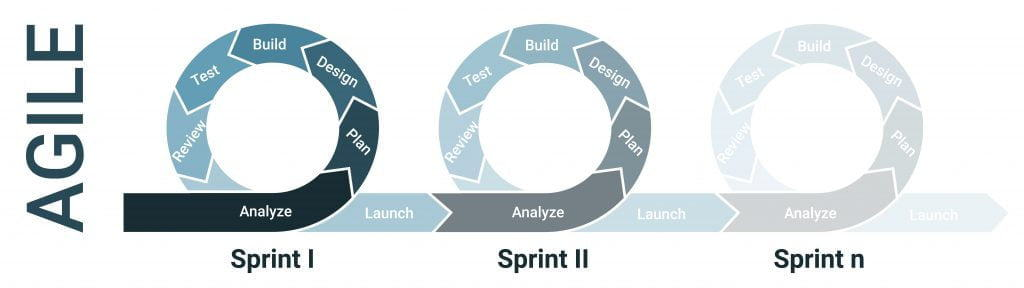
\includegraphics[width=0.8\textwidth]{agile.jpeg}
    \caption{Agile Methodology}
    \label{fig:agile}
\end{figure}

Given our need for flexibility and continuous client engagement, we adopted the \textbf{Agile} methodology \cite{atlassian_agile} as our primary project management framework. This approach allowed us to break down the project into manageable iterations, or sprints, rather than adhering to a rigid, linear timeline. To facilitate this, we leveraged \textbf{Jira} \cite{atlassian_jira}, a powerful project management tool. Jira enabled us to create and assign tasks, manage our sprints, and conduct thorough sprint reviews. This process provided our team with clear visibility into the development pipeline and ensured that we were consistently delivering value. Furthermore, we integrated a \textbf{Continuous Integration} (CI)\cite{atlassian_ci}. This allowed us to automate the building, testing, and deployment of our code, ensuring that new features and bug fixes could be released efficiently and reliably. This combination of an Agile workflow, supported by Jira and automated through CI, allowed us to maintain a dynamic and responsive development process that could quickly adapt to new requirements and feedback.

Our team operated with an independent, decentralized structure where each member took ownership of their assigned tasks. This platform provided a transparent view of our progress and allowed us to manage our workload effectively. Our team maintained a consistent communication cadence with weekly meetings every Monday to review sprint progress, address any roadblocks, and plan the upcoming week's tasks. Furthermore, we held meetings with the client every Friday, which served as dedicated sessions for feature demos, gathering feedback, and addressing any questions or new requests. To tackle complex tickets that required collaborative effort, we also adopted pair programming on other weekdays. This practice not only facilitated the resolution of challenging technical issues but also promoted knowledge sharing and code quality across the team.

    
\section{Technologies and Tools}
    \subsection{Programming Languages}
        The primary programming language for the backend was Java 21 \cite{oracle_java21}, chosen for its stability, performance, and extensive ecosystem. On the frontend, we used TypeScript \cite{typescript}, which provided a robust, type-safe environment for developing the user interface and ensured a higher level of code quality and maintainability.
    \subsection{Frameworks and Libraries}
        For the backend, we used the Spring Boot \cite{spring_boot} framework, which simplified the creation of a production-ready, microservices-based \cite{microservices_io} system. This framework's convention-over-configuration approach allowed us to rapidly develop and deploy various services, including those for location data, translation, and navigation.

        On the frontend, the Next.js \cite{nextjs} framework was used to build the user interface. Next.js was selected for its server-side rendering (SSR) \cite{epam_ssr} and static site generation capabilities, which improved application performance and search engine optimization (SEO). We utilized DaisyUI \cite{daisyui}, a component library for Tailwind CSS \cite{tailwindcss}, to accelerate the styling and design process, ensuring a consistent and modern look and feel.
    \subsection{Databases}
        The project utilized two primary databases to handle different data requirements. PostgreSQL \cite{postgresql} was used as the main relational database for storing structured data, such as user information and core application data, due to its reliability and ACID \cite{mongodb_acid} compliance. For real-time, unstructured data and caching, we employed Redis, a high-performance in-memory data store. Additionally, Elastic Search was integrated for efficient searching of points of interest within the virtual tour, providing users with quick and relevant results.
    \subsection{Version Control}
        We managed our source code and collaborative development process using \textbf{Git} \cite{git} and \textbf{GitHub} \cite{github}. Git provides a decentralized version control system, allowing each team member to work on their own branches independently. GitHub served as the centralized repository, enabling seamless code reviews, issue tracking, and a clear history of all project changes. This setup, combined with our Continuous Integration (CI) pipeline, ensured that our codebase remained stable and up-to-date.

% \section{Data Collection and Analysis}

%     \subsection{Data Sources}



%     \subsection{Data Processesing}

    
